% =====================================================
\chapter{Foundational Experiments}
\label{chap:foundational_experiments}

This chapter presents some foundational experiments conducted to get used to the sensing technologies needed as part of the Digital Twin.
% =====================================================
\section{RFID Experiments}
\label{sec:RFID_experiments}

A contactless technology called RFID (Radio Frequency Identification) is utilized for data collection and automatic identification. It eliminates the need for physical contact by using radio waves to transport data between an RFID tag and a reader. RFID tags and RFID readers are the two fundamental parts of an RFID system. A tiny electronic device called an RFID tag is affixed to the item you wish to track or identify. The tag is made up of an antenna that connects to the reader and a microchip that saves data. Active and passive RFID tags are two different categories.

Based on the MFRC522 chip created by NXP Semiconductors, the RC522 RFID module is a popular and inexpensive RFID reader/writer module. The standard frequency for RFID communication, 13.56 MHz, is where it operates.

This module supports several communication protocols, such as SPI (Serial Peripheral Interface), I2C (Inter-Integrated Circuit), and UART (Universal Asynchronous Receiver-Transmitter), and is appropriate for short-distance communication, usually within a 5 cm range.

The majority of RC522 modules include:

  a)  A 1K RFID card from MIFARE Classic
  b)  A key fob or tag

\begin{figure}[!h]
    \centering
    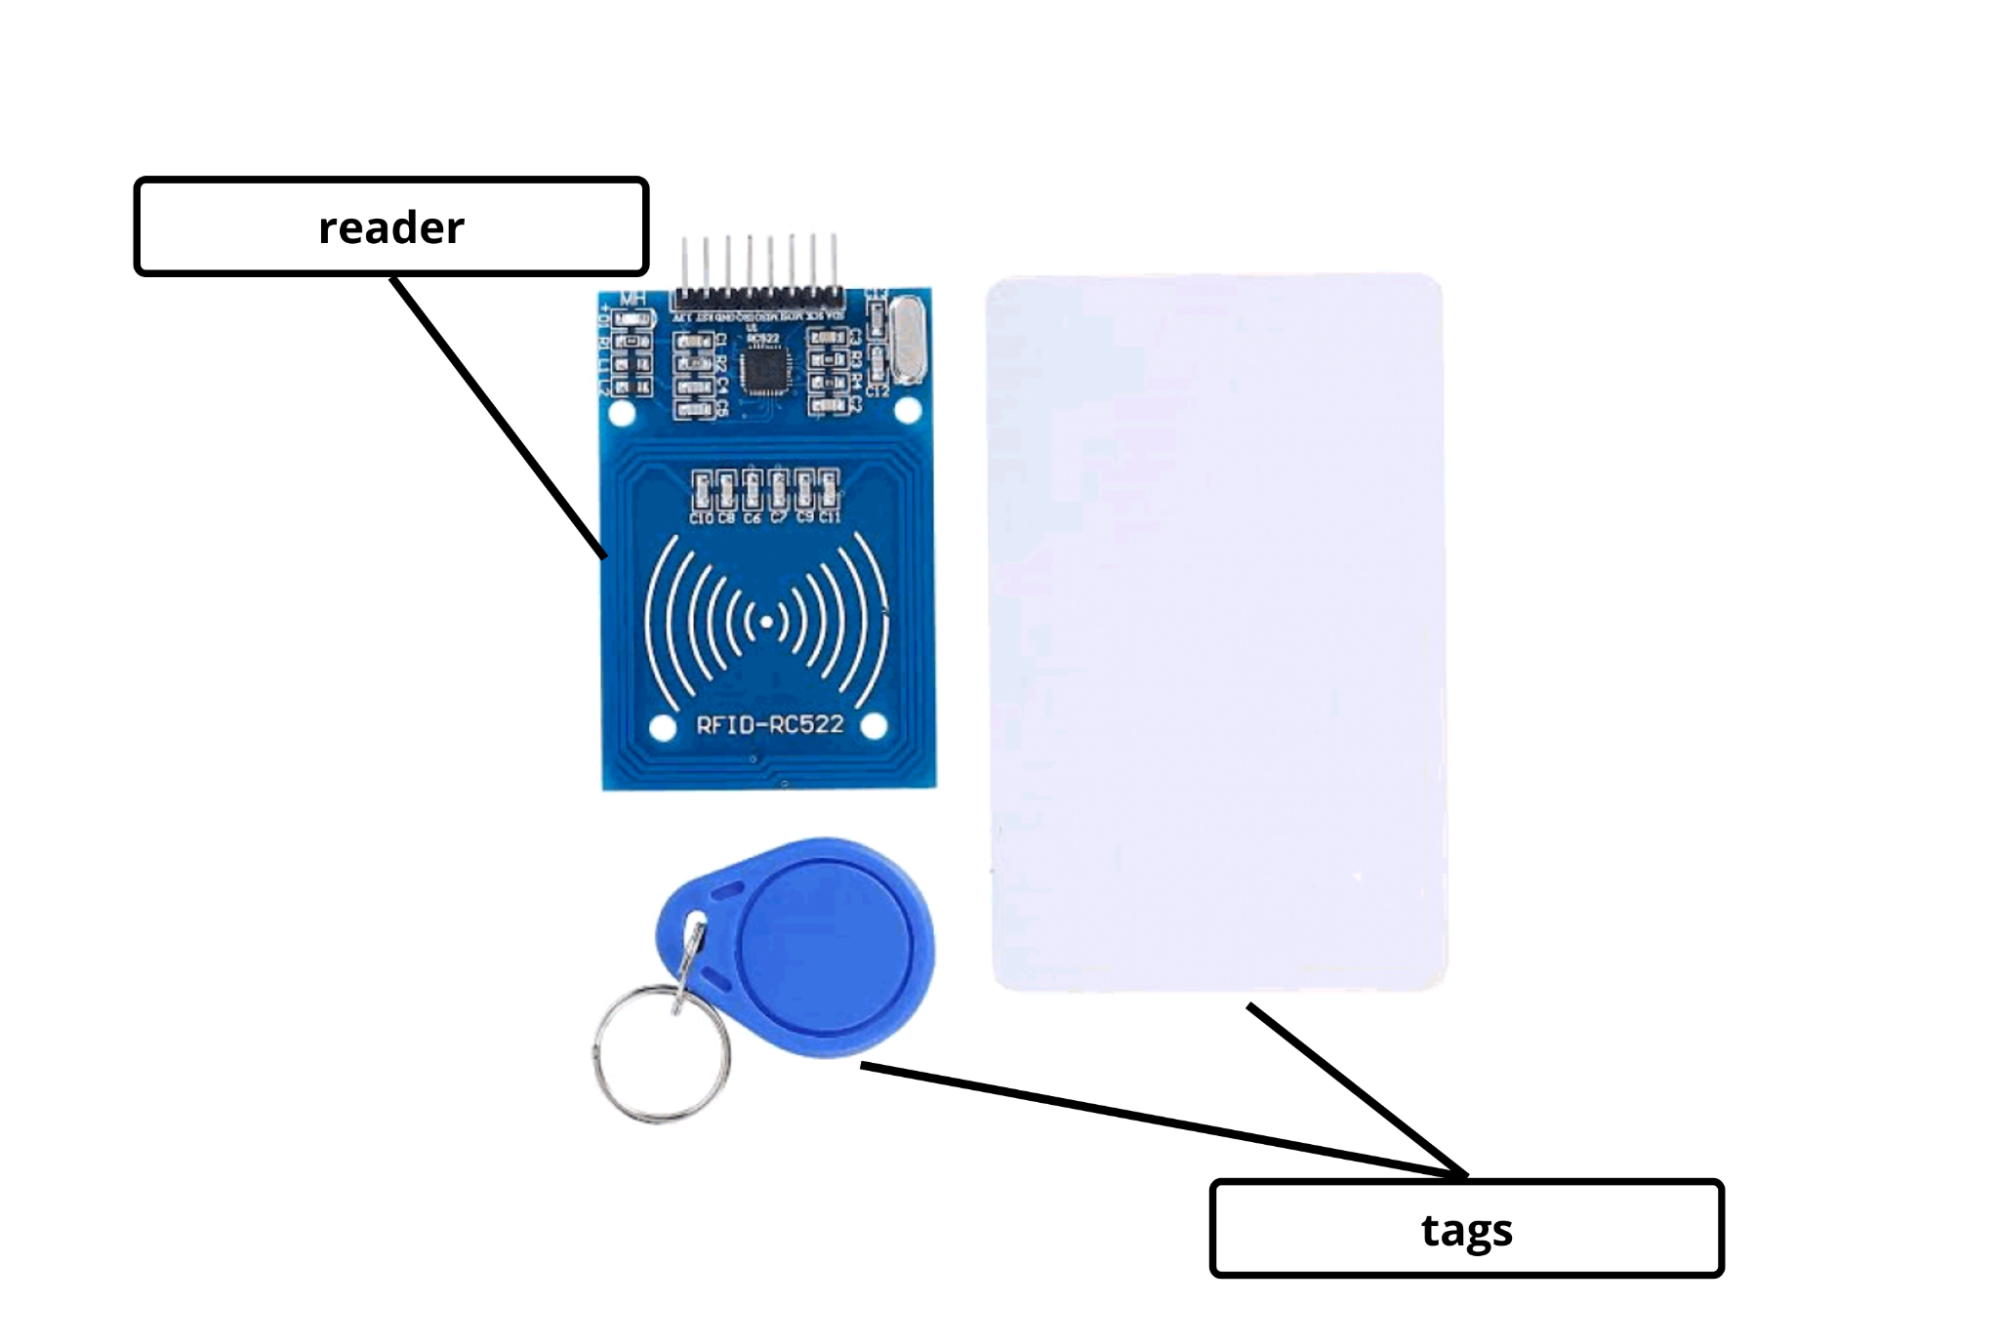
\includegraphics[width=0.65\linewidth]{images/RFID.png}
    \caption{RFID tag and reader}
    \label{fig:RFID}
\end{figure}

% =====================================================
\section{PIR sensor experiments}
\label{sec:PIR_experiment}

An electronic sensor that detects infrared (IR) light emitted by objects within its field of vision is called a passive infrared sensor (PIR sensor). PIR-based motion detectors are the most common application for them. PIR sensors are frequently utilized in automated lighting and security alarm systems. 
\begin{figure}[!h]
    \centering
    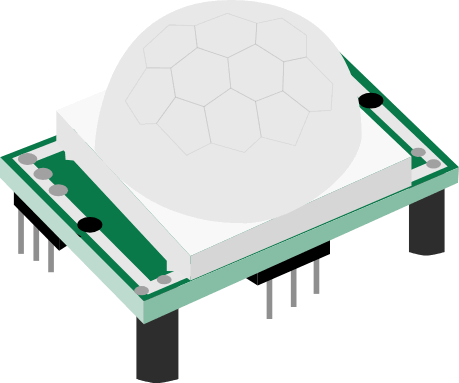
\includegraphics[width=0.55\linewidth]{images/PIR.png}
    \caption{}
    \label{fig:PIR sensor}
\end{figure}

% =====================================================
\section{Ultrasonic Sensor Experiments}
\label{sec:ultrasonic_experiments}

The ultrasonic sensor uses sound waves and the echo principle to calculate distance from obstacles. 
Distance Travelled = \frac{Speed of Sound \multiply Time Travlled}{2}
HCSR04 is the code for an ultrasonic sensor module avaialable in the market. It has a range from 2cm to 400cm. The ranging accuracy is 3mm. The sensor module has four pins: VCC, GND, TRIG and
ECHO.
\begin{figure}[!h]
    \centering
    \includegraphics[width=0.65\linewidth]{images/hcsr04.jpg}
    \caption{Ultrasonic sensor module}
    \label{fig:ddpm_samples}
\end{figure}

% =====================================================
\section{Summary of Foundational Experiments}
\label{sec:foundational_summary}

Through the above experiments, an idea of different Physical to Virtual (P2V) experiments was evaluated.
